\subsubsection{Description/circuitry}
% Describe the concept and circuitry of the latching/reset system for a tripped IMD or AMS.  Describe the method for resetting the IMD and AMS.
The \gls{ams} and \gls{imd} error is latched in the \gls{ecua} circuitry. The \gls{sdc} is switched by Q$_2$ and Q$_3$ respectively. Both \gls{ams} and \gls{imd} states are positive logic (AMS\_OK and IMD\_OK), combined using th first U$_2$ gate. If either of the two signals goes to zero (\gls{imd} error or \gls{ams} error), the output of U$_2$ goes high. That triggers the latching circuit comprised of Q$_4$ and Q$_5$. Q$_4$ and Q$_5$ forms a classic thyristor structure, that can be reset only by a power cycle.  There is a few seconds delay introduced in the latch activation by U$_1$ and the RC timing network. This is to accommodate for the \gls{imd} and \gls{ams} self-test/start-up routines, when the AMS\_OK and IMD\_OK signals are not yet asserted. During this delay, the \gls{sdc} is forced open by the action of U$_4$. It is therefore not possible to start the car (\gls{sdc} open) during the self-test/start-up time, when the latch is disabled.
5 V power for this circuit is derived from the 24 V \gls{glvs}, after \gls{glvms}, using a linear regulator.


\subsubsection{Wiring/cables/connectors}
%Describe wiring, show schematics, describe connectors and cables used and show useful data regarding the wiring.  If not detailed in section 2.1, be sure to show how the device opens the shutdown circuit.
% SDC monitoring scheme
Whole latching circuit is implemented in \gls{ecua}.


\subsubsection{Position in car}
%Provide CAD-renderings showing the relevant parts. Mark the parts in the rendering, if necessary.
\Gls{imd} and \gls{ams} error latch is placed in \gls{ecua} on the back of car. See \ref{fig:ECUA}.

\begin{figure}[H]
	\centering
	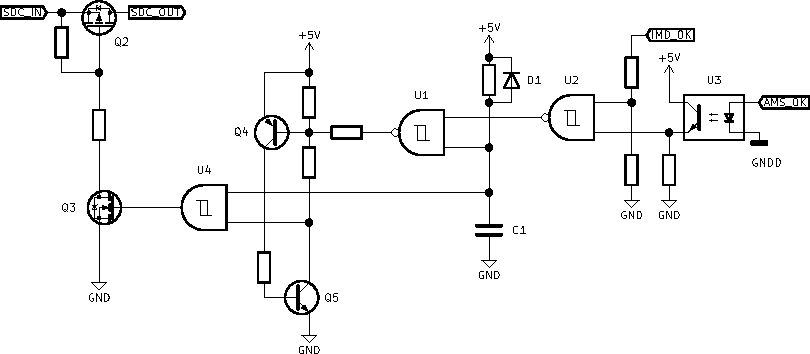
\includegraphics[width=\textwidth]{./img/ECUA_imd_ams_latch.pdf}
	\caption{\Gls{ams} \gls{imd} latch schematic.}
	\label{}
\end{figure}